\chapter{ВЧ-моделирование}

Пользуясь спроектированными ранее элементами составим общую схему приёмной ячейки по примеру структурной схемы из технического задания (Рис.~\ref{fig:receiving_cell_schematic}).

\begin{figure}[!ht]
    \centering
    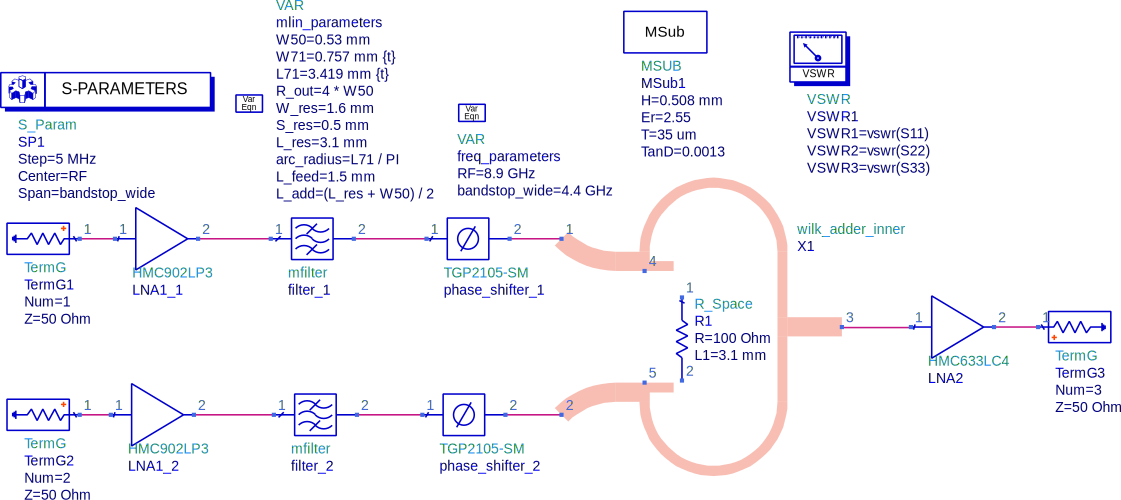
\includegraphics[width=\textwidth]{receiving_cell_schematic.pdf}
    \caption{Схема проектируемой приёмной ячейки}%
    \label{fig:receiving_cell_schematic}
\end{figure}

Проведём моделирование и выведем зависимость КСВН от частоты (Рис.~\ref{fig:receiving_cell_data_VSWR})и АЧХ (Рис.~\ref{fig:receiving_cell_data_response}).

\begin{figure}[!ht]
    \centering
    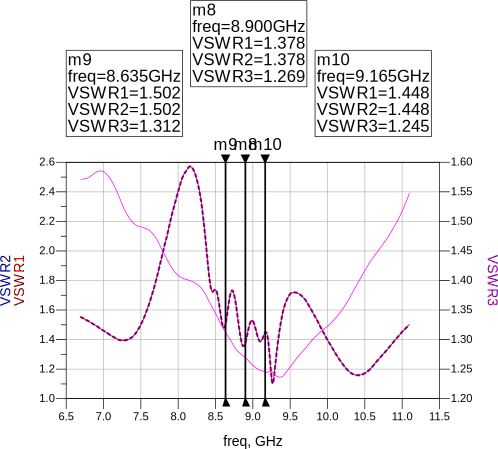
\includegraphics[width=\textwidth]{receiving_cell_data_VSWR.pdf}
    \caption{Зависимость КСВН проектируемой приёмной ячейки от частоты}%
    \label{fig:receiving_cell_data_VSWR}
\end{figure}

\begin{figure}[!ht]
    \centering
    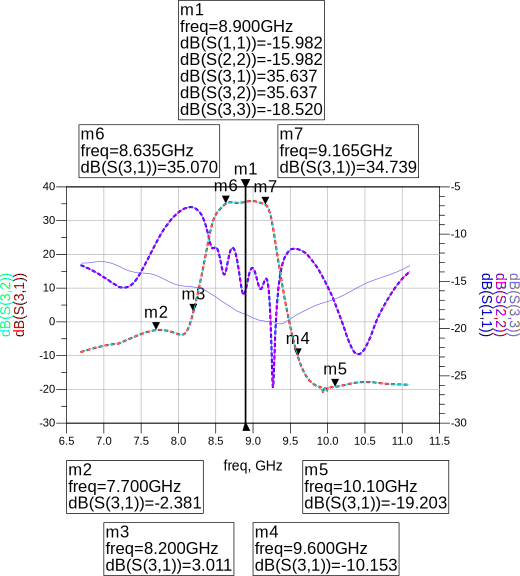
\includegraphics[width=\textwidth]{receiving_cell_data_response.pdf}
    \caption{АЧХ проектируемой приёмной ячейки}%
    \label{fig:receiving_cell_data_response}
\end{figure}

По результатам моделирования можно сделать вывод, что в целом приёмная ячейка удовлетворяет техническому заданию, однако стоит отметить отрицательные стороны выполненного дизайна:
\begin{itemize}
    \item
        КСВН в полосе пропускания в некоторых точках выходит за установленный предел в $1.5$;
    \item
        выбранные цепи согласования скорее всего не являются оптимальным выбором, т.к. имеют весьма большие габариты и увеличивают потери.
\end{itemize}
